\documentclass[11pt]{article}
\usepackage[paperwidth=220mm,paperheight=320mm,left=16mm,right=16mm,top=18mm,bottom=18mm,headheight=16pt,headsep=10pt,footskip=14pt]{geometry}
\usepackage{fix-cm}
\usepackage{fontspec,amsmath,amssymb,graphicx,array}
\usepackage[unicode,hidelinks]{hyperref}
\usepackage{polyglossia}
\setmainlanguage{latin}
\setotherlanguages{arabic,greek}
\setmainfont{Linux Libertine O}[Ligatures=TeX]
\newfontfamily\greekfont{FreeSerif}[Script=Greek]
\newfontfamily\arabicfont{Amiri}[Script=Arabic]
\graphicspath{{../source/presentation/}}
\hypersetup{pdftitle={Al-Battani, Opus astronomicum. Nallino Latin source. S02 v009},pdfauthor={Al-Battani; Carlo Alfonso Nallino (Latin translation and notes)}}
\makeatletter
\def\ps@sourceedition{%
\def\@oddhead{\vbox{\hbox to\textwidth{\fontsize{8}{10}\selectfont C. A. NALLINO — VERSIO ET ADNOTATIONES\hfil\leftmark}\vskip3pt\hrule height.25pt}}%
\let\@evenhead\@oddhead
\def\@oddfoot{\hbox to\textwidth{\fontsize{7}{9}\selectfont\rightmark\hfil\thepage}}%
\let\@evenfoot\@oddfoot}
\makeatother
\pagestyle{sourceedition}
\setlength{\parindent}{0pt}\setlength{\parskip}{0pt}
\newcommand{\sourceglyph}[1]{\raisebox{-.17em}{\includegraphics[height=1.23em]{#1.png}}}
\newsavebox{\sourcelinebox}
\newcommand{\SourceLine}[2]{\sbox{\sourcelinebox}{\strut #2}%
\ifdim\wd\sourcelinebox>\linewidth\typeout{SOURCEWIDTH|#1|\the\wd\sourcelinebox|\the\linewidth}\fi%
\noindent\hypertarget{#1}{}#2\strut\par}
\newcommand{\BeginSource}[2]{\clearpage\markboth{PAG. #2}{#1}\hypertarget{#1}{}\pdfbookmark[0]{#1 — p. #2}{bk-#1}\fontsize{11.1}{13.8}\selectfont}
\tracinglostchars=2

\newcommand{\qfrac}[2]{{}^{#1}\!/_{{#2}}}
\newcommand{\Name}[1]{{\addfontfeatures{LetterSpace=4.0}#1}}
\newcommand{\Indent}{\hspace*{1.6em}}
\newcommand{\CenterLine}[1]{\makebox[\linewidth][c]{{\fontsize{12}{15}\selectfont #1}}}
\newlength{\FullSourceWidth}\newlength{\GutterOffset}\newif\ifNumbersLeft
\newcommand{\DSource}[2]{\BeginSource{AB01-PDF#1}{#2}%
 \setlength{\FullSourceWidth}{\textwidth}\setlength{\GutterOffset}{0pt}%
 \ifodd#2\relax\NumbersLefttrue\else\NumbersLeftfalse\fi}
\newsavebox{\DLBox}
\newcommand{\DLine}[4]{%
 \par\noindent\hypertarget{#1}{}%
 \ifx\relax#2\relax\else
   \ifNumbersLeft
    \rlap{\kern-\GutterOffset\llap{\fontsize{7}{8}\selectfont #2\hspace{3mm}}}%
   \else
    \rlap{\kern\dimexpr\FullSourceWidth-\GutterOffset\relax\hspace{3mm}{\fontsize{7}{8}\selectfont #2}}%
   \fi
 \fi
 \ifx\relax#3\relax\else
   \ifNumbersLeft
    \rlap{\kern\dimexpr\FullSourceWidth-\GutterOffset\relax\hspace{3mm}{\fontsize{7}{8}\selectfont #3}}%
   \else
    \rlap{\kern-\GutterOffset\llap{\fontsize{7}{8}\selectfont #3\hspace{3mm}}}%
   \fi
 \fi
 \sbox{\DLBox}{\strut #4}%
 \ifdim\wd\DLBox>\linewidth\typeout{DIPLOMATICWIDTH|#1|\the\wd\DLBox|\the\linewidth}\fi
 \usebox{\DLBox}\strut\par}

\begin{document}
\setcounter{page}{44}
\DSource{0133}{44}
\hypertarget{AB01-PDF0133-P01}{}
\DLine{AB01-PDF0133-body-L001}{}{}{partem quam Sol medio suo itinere ab initio Arietis ad initium Librae percurrit, scilicet, ut}
\DLine{AB01-PDF0133-body-L002}{}{}{supra vidimus, $183^\circ56'12''$. Arcus KLRM, semicircumferentia excentrici, $180^\circ$ continet; quis-}
\DLine{AB01-PDF0133-body-L003}{}{}{que igitur arcuum PK, YM est dimidia pars eorum $3^\circ56'12''$, quibus Sol medio suo itinere}
\DLine{AB01-PDF0133-body-L004}{}{}{$180^\circ$ superat, idest $1^\circ58'6''$. --- Manifestum etiam est arcum PKLR (1) excentrici id esse quod}
\DLine{AB01-PDF0133-body-L005}{5}{}{Sol, medio suo itinere, ab initio Arietis ad initium Cancri percurrit; igitur $92^\circ14'10''$ erit;}
\DLine{AB01-PDF0133-body-L006}{}{}{et quia arcus PKL, ob ea quae nuper diximus, $91^\circ58'6''$ complectitur, arcus LR $0^\circ16'4''$}
\DLine{AB01-PDF0133-body-L007}{}{}{continebit. Item manifestum est perpendicularem PQ sinum esse arcus PK, et perpendicula-}
\DLine{AB01-PDF0133-body-L008}{}{}{rem RG sinum arcus LR; igitur PQ fere $2^p3'39''$, et RG fere $0^p16'45''$ erit. Quoniam}
\DLine{AB01-PDF0133-body-L009}{}{}{linea KM parallela est lineae AC, erit linea ES aequalis PQ; et similiter, quia LN parallela}
\DLine{AB01-PDF0133-body-L010}{10}{}{est lineae BD, erit FS aequalis RG. Est itaque etiam latus EF trianguli rectanguli ESF no-}
\DLine{AB01-PDF0133-body-L011}{}{}{tum; quadratum lateris ES est fere $4^p14'48''$, quadratum lateris FS fere $0^p4'41''$, summa}
\DLine{AB01-PDF0133-body-L012}{}{}{igitur $4^p19'29''$ (2) efficit quadratum lateris EF, cuius radix $2^p4'\,\qfrac{3}{4}$ est quantitas lineae EF}
\DLine{AB01-PDF0133-body-L013}{}{}{ambo centra coniungentis. Ea ratione autem, qua quadrans circuli triangulum rectangulum}
\DLine{AB01-PDF0133-body-L014}{}{}{ESF circumdantis $90^\circ$ complectitur, et semidiametrus $60^p$, erit arcus EF circiter $1^\circ59'$ (3); et}
\DLine{AB01-PDF0133-body-L015}{15}{}{haec est maxima anomalia motus Solis per has observationes manifesta ({\itshape b}).}
\hypertarget{AB01-PDF0133-P02}{}
\DLine{AB01-PDF0133-body-L016}{}{}{\Indent Nunc in quantitatem arcus BH eclipticae inquiramus; qua cognita, etiam arcus HA reli-}
\DLine{AB01-PDF0133-body-L017}{}{p. 67.}{quus notus erit. Punctum T est locus apogei in circulo Solis excentrico; nam, si lineam EF,}
\DLine{AB01-PDF0133-body-L018}{}{}{ambo centra coniungentem, usque ad eclipticam producimus, ipsa circulum KLMN in T, et}
\DLine{AB01-PDF0133-body-L019}{}{}{circulum eclipticae in H secat. Necesse est ut rationem lineae EF ad semidiametrum EH co-}
\DLine{AB01-PDF0133-body-L020}{20}{}{gnoscamus, nec non quantitatem arcus BH eclipticae. Iam vidimus lineam EF $2^p4'\,\qfrac{3}{4}$ com-}
\DLine{AB01-PDF0133-body-L021}{}{}{plecti ea ratione qua semidiametrus $60^p$ continet; eadem ratione igitur linea EH, quae, ut EB,}
\DLine{AB01-PDF0133-body-L022}{}{}{semidiametrus est, lineam EF 28 vicibus et $\qfrac{5}{6}$ fere continebit. Quoniam linea FS, ut dixi-}
\DLine{AB01-PDF0133-body-L023}{}{}{mus, [$0^p16'45''$] est, si linea EF $60^p$ ponatur, erit iuxta hanc rationem linea FS circiter $8^p4'$;}
\par\noindent\begin{minipage}[t]{0.46\FullSourceWidth}\vspace{0pt}\centering\hypertarget{AB01-PDF0133-F01}{}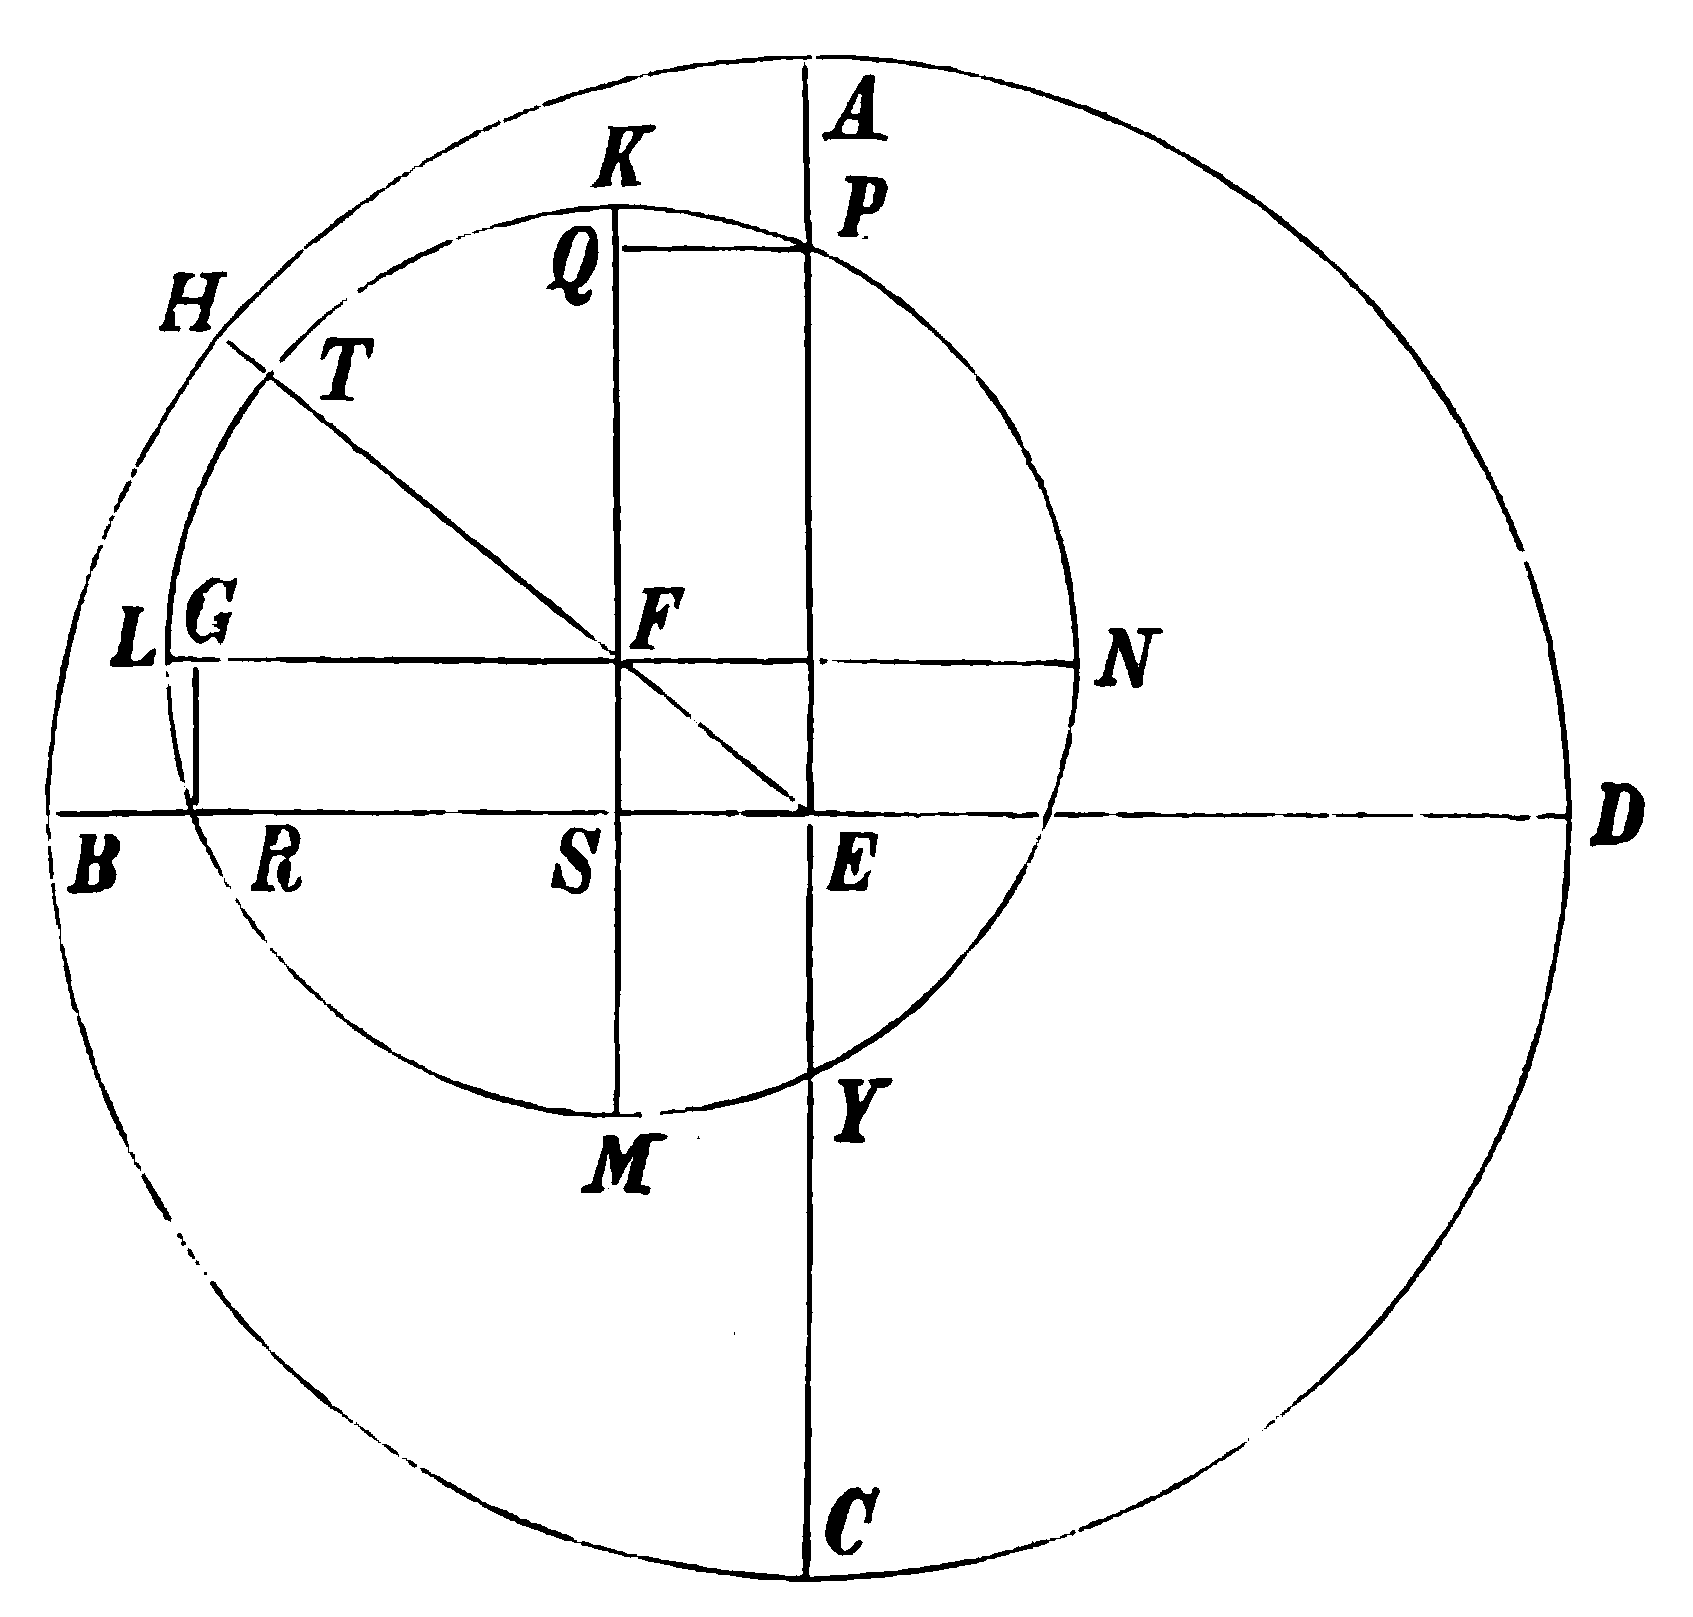
\includegraphics[width=\linewidth]{AB01-PDF0133-F01.png}\end{minipage}\hfill\begin{minipage}[t]{0.5\FullSourceWidth}\vspace{0pt}\setlength{\GutterOffset}{0.5\FullSourceWidth}
\DLine{AB01-PDF0133-body-L024}{}{}{hoc enim invenitur si $28\,\qfrac{5}{6}$ vicibus [$0^p16'45''$]}
\DLine{AB01-PDF0133-body-L025}{25}{}{multiplicantur. --- Aut, si mavis, lineam FS in}
\DLine{AB01-PDF0133-body-L026}{}{}{semidiametrum EH multiplica; invenies $16^p45'$,}
\DLine{AB01-PDF0133-body-L027}{}{}{quae, per lineam EF scilicet per $2^p4'\,\qfrac{3}{4}$ divisa,}
\DLine{AB01-PDF0133-body-L028}{}{}{dabunt $8^p4'$, quod est [sinus] anguli BEH; ar-}
\DLine{AB01-PDF0133-body-L029}{}{}{cus igitur BH $7^\circ43'$ circiter continet. Itaque}
\DLine{AB01-PDF0133-body-L030}{30}{}{manifestum est punctum T apogei in excentrico,}
\DLine{AB01-PDF0133-body-L031}{}{}{a puncto solstitii aestivi versus partem anterio-}
\DLine{AB01-PDF0133-body-L032}{}{}{rem signorum $7^\circ43'$ distare, scilicet $82^\circ17'$ ab}
\DLine{AB01-PDF0133-body-L033}{}{}{initio Arietis esse. Hoc invenire volebamus. Ob-}
\DLine{AB01-PDF0133-body-L034}{}{}{servatio iuxta quam hunc calculum fecimus,}
\DLine{AB01-PDF0133-body-L035}{35}{}{anno 1194 aerae Dhū ’l-qarnayn (4) fuit, quo}
\DLine{AB01-PDF0133-body-L036}{}{}{iter Solis ab initio Arietis ad initium Cancri et}
\DLine{AB01-PDF0133-body-L037}{}{}{ad initium Librae observavimus ({\itshape c}).}
\hypertarget{AB01-PDF0133-P03}{}
\DLine{AB01-PDF0133-body-L038}{}{}{\Indent Restat nunc nobis ut hanc anomaliam ad}\end{minipage}\par
\DLine{AB01-PDF0133-body-L039}{}{}{gradus eclipticae distribuamus, et portiones eius quae ad singulos gradus pertinent in tabulis}
\par\vspace{6pt}\hrule height.25pt\vspace{5pt}
\noindent\begin{minipage}[t]{.48\textwidth}\vspace{0pt}\fontsize{9}{11.5}\selectfont\setlength{\GutterOffset}{0pt}
\hypertarget{AB01-PDF0133-N01}{}
\DLine{AB01-PDF0133-notes_left-L001}{}{}{\Indent (1) Male codex PKL.}
\hypertarget{AB01-PDF0133-N02}{}
\DLine{AB01-PDF0133-notes_left-L002}{}{}{\Indent (2) Male secundae apud Platonem $59''$.}
\hypertarget{AB01-PDF0133-N03}{}
\DLine{AB01-PDF0133-notes_left-L003}{}{}{\Indent (3) Plato male $1^\circ58'$; \Name{Ibn Yūnus} (apud \Name{Caus-}}
\DLine{AB01-PDF0133-notes_left-L004}{}{}{\Name{sin}, {\itshape Le livre de la grande table Hakémite}, in}
\DLine{AB01-PDF0133-notes_left-L005}{}{}{Notices et extraits des mss. de la Bibl. Nation., t. VII,}
\DLine{AB01-PDF0133-notes_left-L006}{}{}{Paris 1804, p. 155) scribit: « al-Battānī aequationem}
\DLine{AB01-PDF0133-notes_left-L007}{}{}{« totam Solis calculavit, invenitque $1^\circ59'10''$ esse ».}
\end{minipage}
\hfill\begin{minipage}[t]{.48\textwidth}\vspace{0pt}\fontsize{9}{11.5}\selectfont\setlength{\GutterOffset}{0pt}
\DLine{AB01-PDF0133-notes_right-L001}{}{}{\Name{Halley} p. 917, et \Name{Delambre}, {\itshape Astr. moyen âge},}
\DLine{AB01-PDF0133-notes_right-L002}{}{}{p. 36, qui hodiernis tabulis trigonometricis usi sunt,}
\DLine{AB01-PDF0133-notes_right-L003}{}{}{invenere quoque $1^\circ59'10''$. Codicis lectio igitur bona}
\DLine{AB01-PDF0133-notes_right-L004}{}{}{est; in tabulis aequationis Solis (fol. 191,r.) re vera}
\DLine{AB01-PDF0133-notes_right-L005}{}{}{maxima aequatio est $1^\circ59'10''$.}
\hypertarget{AB01-PDF0133-N04}{}
\DLine{AB01-PDF0133-notes_right-L006}{}{}{\Indent (4) Incipit, iuxta usum auctoris nostri, die 1 Se-}
\DLine{AB01-PDF0133-notes_right-L007}{}{}{ptembris 882 post Chr. n.}
\end{minipage}

\DSource{0134}{45}
\hypertarget{AB01-PDF0134-P01}{}
\DLine{AB01-PDF0134-body-L001}{}{}{describamus, ut facile possit aequatio motus Solis inveniri. Ostendit Ptolemaeus (1) motus va-}
\DLine{AB01-PDF0134-body-L002}{}{p. 68.}{rios duobus modis effingi posse; quorum alter est ut ponatur planetam habere circulum eclip-}
\DLine{AB01-PDF0134-body-L003}{}{}{ticae concentricum, super quem alius circulus sit, cuius centrum circumferentiam primi per-}
\DLine{AB01-PDF0134-body-L004}{}{}{currat. Hic secundus circulus est circulus minor, Terram non ambiens, cuius centrum circulus}
\DLine{AB01-PDF0134-body-L005}{5}{}{maior rotare facit versus partem successionis signorum iuxta quantitatem motus longitudinalis}
\DLine{AB01-PDF0134-body-L006}{}{}{planetae versus partem in quam signa succedunt. Sidus ipsum in epicyclo, qui est circulus}
\DLine{AB01-PDF0134-body-L007}{}{}{minor, versus praecedentem aut versus subsequentem partem movetur; aut circulus minor}
\DLine{AB01-PDF0134-body-L008}{}{}{planetam versus alterutram partem rotare facit. Hic est motus anomaliae quae ad planetam}
\DLine{AB01-PDF0134-body-L009}{}{}{pertinet. --- Alter explicandi modus est ut ponatur sidus habere circulum concentricum ecli-}
\DLine{AB01-PDF0134-body-L010}{10}{}{pticae, et alterum excentricum sed illi aequalem, qui eum duobus locis secet Planeta est in}
\DLine{AB01-PDF0134-body-L011}{}{}{excentrico, sive hic eum movet, sive ipse in excentrico movetur. --- Utraque ratio anomaliam}
\DLine{AB01-PDF0134-body-L012}{}{}{pariter explicat; nos a prima incipiemus.}
\hypertarget{AB01-PDF0134-P02}{}
\DLine{AB01-PDF0134-body-L013}{}{}{\Indent Circulum ABCD eclipticae circa centrum E describamus; sit A, initio, centrum epicycli}
\DLine{AB01-PDF0134-body-L014}{}{}{HF (2). Diametrum AC usque ad H producamus, quod est punctum apogei in epicyclo; sit F}
\DLine{AB01-PDF0134-body-L015}{15}{}{locus Solis in epicyclo, et ab eo perpendicularem supra lineam AH usque ad punctum M du-}
\DLine{AB01-PDF0134-body-L016}{}{}{camus; denique lineam AF signemus, lineae AH aequalem, nam ambae sunt semidiametri}
\DLine{AB01-PDF0134-body-L017}{}{}{epicycli. Ob ea quae in hoc ipso capite iam diximus, patet eam $2^p4'\,\qfrac{3}{4}$ complecti, ut semi-}
\DLine{AB01-PDF0134-body-L018}{}{}{diametrum EF epicycli in figura praecedenti. Quo cognito, motum Solis in epicyclo versus}
\DLine{AB01-PDF0134-body-L019}{}{}{partem contrariam successioni signorum observa, vel quantitatem qua epicyclus motu medio}
\DLine{AB01-PDF0134-body-L020}{20}{}{diurno Solem versus illam partem movet, iuxta rationem qua circumferentia epicycli in $360^\circ$}
\DLine{AB01-PDF0134-body-L021}{}{}{dividitur. Motus medius Solis, qui observationibus invenitur, est motus centri epicycli versus}
\DLine{AB01-PDF0134-body-L022}{}{p. 69.}{partem successionis signorum; et hic motus quoque ea ratione ponitur qua circulus ABCD}
\DLine{AB01-PDF0134-body-L023}{}{}{$360^\circ$ complectitur.}
\hypertarget{AB01-PDF0134-P03}{}
\DLine{AB01-PDF0134-body-L024}{}{}{\Indent Arcus HF, qui est arcus epicycli inter locum Solis et punctum apogei, $30^\circ$ contineat e}
\DLine{AB01-PDF0134-body-L025}{25}{}{gradibus quorum epicyclus 360 continet. Lineam EF in hac figura ducamus; et in arcum}
\DLine{AB01-PDF0134-body-L026}{}{}{lineae FM, qui est variatio motus Solis eo loco, inquiramus. Linea EA, semidiametrus circuli}
\DLine{AB01-PDF0134-body-L027}{}{}{concentrici eclipticae, 60 partes habet ex iis quarum diametrus AC 120 continet; linea igitur}
\DLine{AB01-PDF0134-body-L028}{}{}{EH, quae centrum circuli parecliptici (3) cum apogeo epicycli coniungit, $62^p4'45''$ erit. Et}
\DLine{AB01-PDF0134-body-L029}{}{}{quia triangulum FMA est rectangulum, quadratum lineae AF erit ut summa quadratorum}
\DLine{AB01-PDF0134-body-L030}{30}{}{AM, FM; angulus autem MAF (4) notus est, ergo etiam linea FM est nota, a qua deinde co-}
\par\vspace{6pt}\hrule height.25pt\vspace{5pt}
\noindent\begin{minipage}[t]{.48\textwidth}\vspace{0pt}\fontsize{9}{11.5}\selectfont\setlength{\GutterOffset}{0pt}
\hypertarget{AB01-PDF0134-N01}{}
\DLine{AB01-PDF0134-notes_left-L001}{}{}{\Indent (1) {\itshape Almag.} III, 3, 4 et 5 (ed. Halma, t. I, p. 170-}
\DLine{AB01-PDF0134-notes_left-L002}{}{}{-183, 183--190, 190--199); quoad Solem tamen hypo-}
\DLine{AB01-PDF0134-notes_left-L003}{}{}{thesim excentrici commodiorem censet.}
\hypertarget{AB01-PDF0134-N02}{}
\DLine{AB01-PDF0134-notes_left-L004}{}{}{\Indent (2) Cod. et Plato HFT; in eorum figura enim}
\DLine{AB01-PDF0134-notes_left-L005}{}{}{punctum T ponitur loco intersectionis epicycli et}
\DLine{AB01-PDF0134-notes_left-L006}{}{}{circuli magni, inter A et D. Sed ex iis quae sequun-}
\DLine{AB01-PDF0134-notes_left-L007}{}{}{tur patet T esse punctum circuli magni indicans di-}
\DLine{AB01-PDF0134-notes_left-L008}{}{}{rectionem apogei.}
\hypertarget{AB01-PDF0134-N03}{}
\DLine{AB01-PDF0134-notes_left-L009}{}{}{\Indent (3) Scilicet paralleli seu concentrici eclipticae.}
\DLine{AB01-PDF0134-notes_left-L010}{}{}{Cum nullum habeat nomen apud scriptores nostra-}
\DLine{AB01-PDF0134-notes_left-L011}{}{}{tes, ita verto Arabicum {\itshape al-mumaththal bi falak}}
\DLine{AB01-PDF0134-notes_left-L012}{}{}{{\itshape al-burūǵ} « similem factum eclipticae » seu {\itshape al-mu-}}
\DLine{AB01-PDF0134-notes_left-L013}{}{}{{\itshape maththal} tantum, qui apud Ptolemaeum interdum}
\DLine{AB01-PDF0134-notes_left-L014}{}{}{\textgreek{ὁ ὁμόκεντρος τῷ κόσμῳ κύκλος} « circulus mundo con-}
\DLine{AB01-PDF0134-notes_left-L015}{}{}{« centricus » vel \textgreek{ὁ ὁμόκεντρος τῷ διὰ μέσων τῶν ζω-}}
\DLine{AB01-PDF0134-notes_left-L016}{}{}{\textgreek{δίων κύκλος} « circulus concentricus circulo per me-}
\end{minipage}
\hfill\begin{minipage}[t]{.48\textwidth}\vspace{0pt}\fontsize{9}{11.5}\selectfont\setlength{\GutterOffset}{0pt}
\DLine{AB01-PDF0134-notes_right-L001}{}{}{dium signorum transeunti » (i. e. eclipticae) vocatur.}
\DLine{AB01-PDF0134-notes_right-L002}{}{}{In astronomia Syriaca Barhebraei vertenda, \Name{Nau}}
\DLine{AB01-PDF0134-notes_right-L003}{}{}{eum {\itshape intersphère de la similitude} appellat; \Name{Golius},}
\DLine{AB01-PDF0134-notes_right-L004}{}{}{in versione al-Farghānī, et \Name{Sédillot}, in versione}
\DLine{AB01-PDF0134-notes_right-L005}{}{}{Ulugh Beg, {\itshape sphaeram} vel {\itshape circulum homocentri-}}
\DLine{AB01-PDF0134-notes_right-L006}{}{}{{\itshape cum}. --- Est circulus concentricus eclipticae in cuius}
\DLine{AB01-PDF0134-notes_right-L007}{}{}{plano iacet; descriptus est in superficie sphaerae}
\DLine{AB01-PDF0134-notes_right-L008}{}{}{Solis vel planetarum, {\itshape al-mumaththal} quoque vo-}
\DLine{AB01-PDF0134-notes_right-L009}{}{}{cata, quae est corpus solidum, concentricum eclip-}
\DLine{AB01-PDF0134-notes_right-L010}{}{}{ticae, duabus superficiebus parallelis contentum, qua-}
\DLine{AB01-PDF0134-notes_right-L011}{}{}{rum exterior superficiem exteriorem sphaerae circuli}
\DLine{AB01-PDF0134-notes_right-L012}{}{}{excentrici (deferentis) in puncto apogeo excentrici}
\DLine{AB01-PDF0134-notes_right-L013}{}{}{tangit; interior superficiem interiorem sphaerae ex-}
\DLine{AB01-PDF0134-notes_right-L014}{}{}{centrici in perigeo. --- Movetur ut signa zodiaci ob}
\DLine{AB01-PDF0134-notes_right-L015}{}{}{praecessionem moventur, ab ortu ad occasum.}
\hypertarget{AB01-PDF0134-N04}{}
\DLine{AB01-PDF0134-notes_right-L016}{}{}{\Indent (4) Cod. HEF.}
\end{minipage}

\DSource{0135}{46}
\hypertarget{AB01-PDF0135-P01}{}
\DLine{AB01-PDF0135-body-L001}{}{}{gnoscitur reliquum latus AM trianguli, quod est [cosinus] arcus FH et anguli FAH (1). Igi-}
\DLine{AB01-PDF0135-body-L002}{}{}{tur est etiam linea EM nota. Cum triangulum FME rectangulum sit, eius hypotenusa EF}
\DLine{AB01-PDF0135-body-L003}{}{}{cognoscitur, ex qua linea FM deprehenditur; arcus autem super FM est arcus anomaliae.}
\hypertarget{AB01-PDF0135-P02}{}
\DLine{AB01-PDF0135-body-L004}{}{}{\Indent Si, ut posuimus, arcus FH $30^\circ$ complectitur, eius sinus erit 30 partium, e partibus qua-}
\DLine{AB01-PDF0135-body-L005}{5}{}{rum semidiametrus AF 60 continet; sed ea ratione qua linea AF $2^p4'45''$ complectitur, erit}
\DLine{AB01-PDF0135-body-L006}{}{}{linea FM $1^p2'22''\,\qfrac{1}{2}$ (2), reliqua igitur AM $1^p48'2''$, et linea EM (3) $61^p48'2''$ (4); unde}
\DLine{AB01-PDF0135-body-L007}{}{}{patet [lineam EF] $61^p48'35''$ circiter esse ({\itshape d}). Sed ex partibus quarum linea EF 60 tantum}
\DLine{AB01-PDF0135-body-L008}{}{}{habet, linea FM $1^p0'33''$ (5) continebit, et arcus super eam positus $0^\circ57'49''$ circiter; et}
\DLine{AB01-PDF0135-body-L009}{}{}{haec est quantitas anomaliae motus Solis, scilicet arcus HF. Est igitur arcus TA eclipticae}
\DLine{AB01-PDF0135-body-L010}{10}{}{$29^\circ2'11''$, qui antea $30^\circ$ erat; nam epicycli centrum a T ad A motum est ut Sol in epicyclo}
\DLine{AB01-PDF0135-body-L011}{}{}{a H ad F.}
\hypertarget{AB01-PDF0135-P03}{}
\DLine{AB01-PDF0135-body-L012}{}{}{\Indent Nunc epicyclum GQP consideremus, cuius centrum est B; locum Solis G ponamus, sit-}
\DLine{AB01-PDF0135-body-L013}{}{p. 70.}{que arcus QG (6), quem Sol a puncto Q apogei percurrit, $150^\circ$ (7); remanent igitur $30^\circ$ arcui}
\DLine{AB01-PDF0135-body-L014}{}{}{PG, qui a loco Solis ad punctum perigei porrigitur. Lineam EG et perpendicularem GK du-}
\DLine{AB01-PDF0135-body-L015}{15}{}{camus; patet triangula BKG et GKE rectangula esse, et latera BG, BE haud ignota; nam}
\DLine{AB01-PDF0135-body-L016}{}{}{BG est semidiametrus epicycli (8), et BE semidiametrus circuli eclipticae. Angulus et arcus}
\DLine{AB01-PDF0135-body-L017}{}{}{GP dati sunt; perpendicularis GK et reliqua linea BK notae; [ergo etiam lineae KE et EG}
\par\noindent\begin{minipage}[t]{0.49\FullSourceWidth}\vspace{0pt}\centering\hypertarget{AB01-PDF0135-F01}{}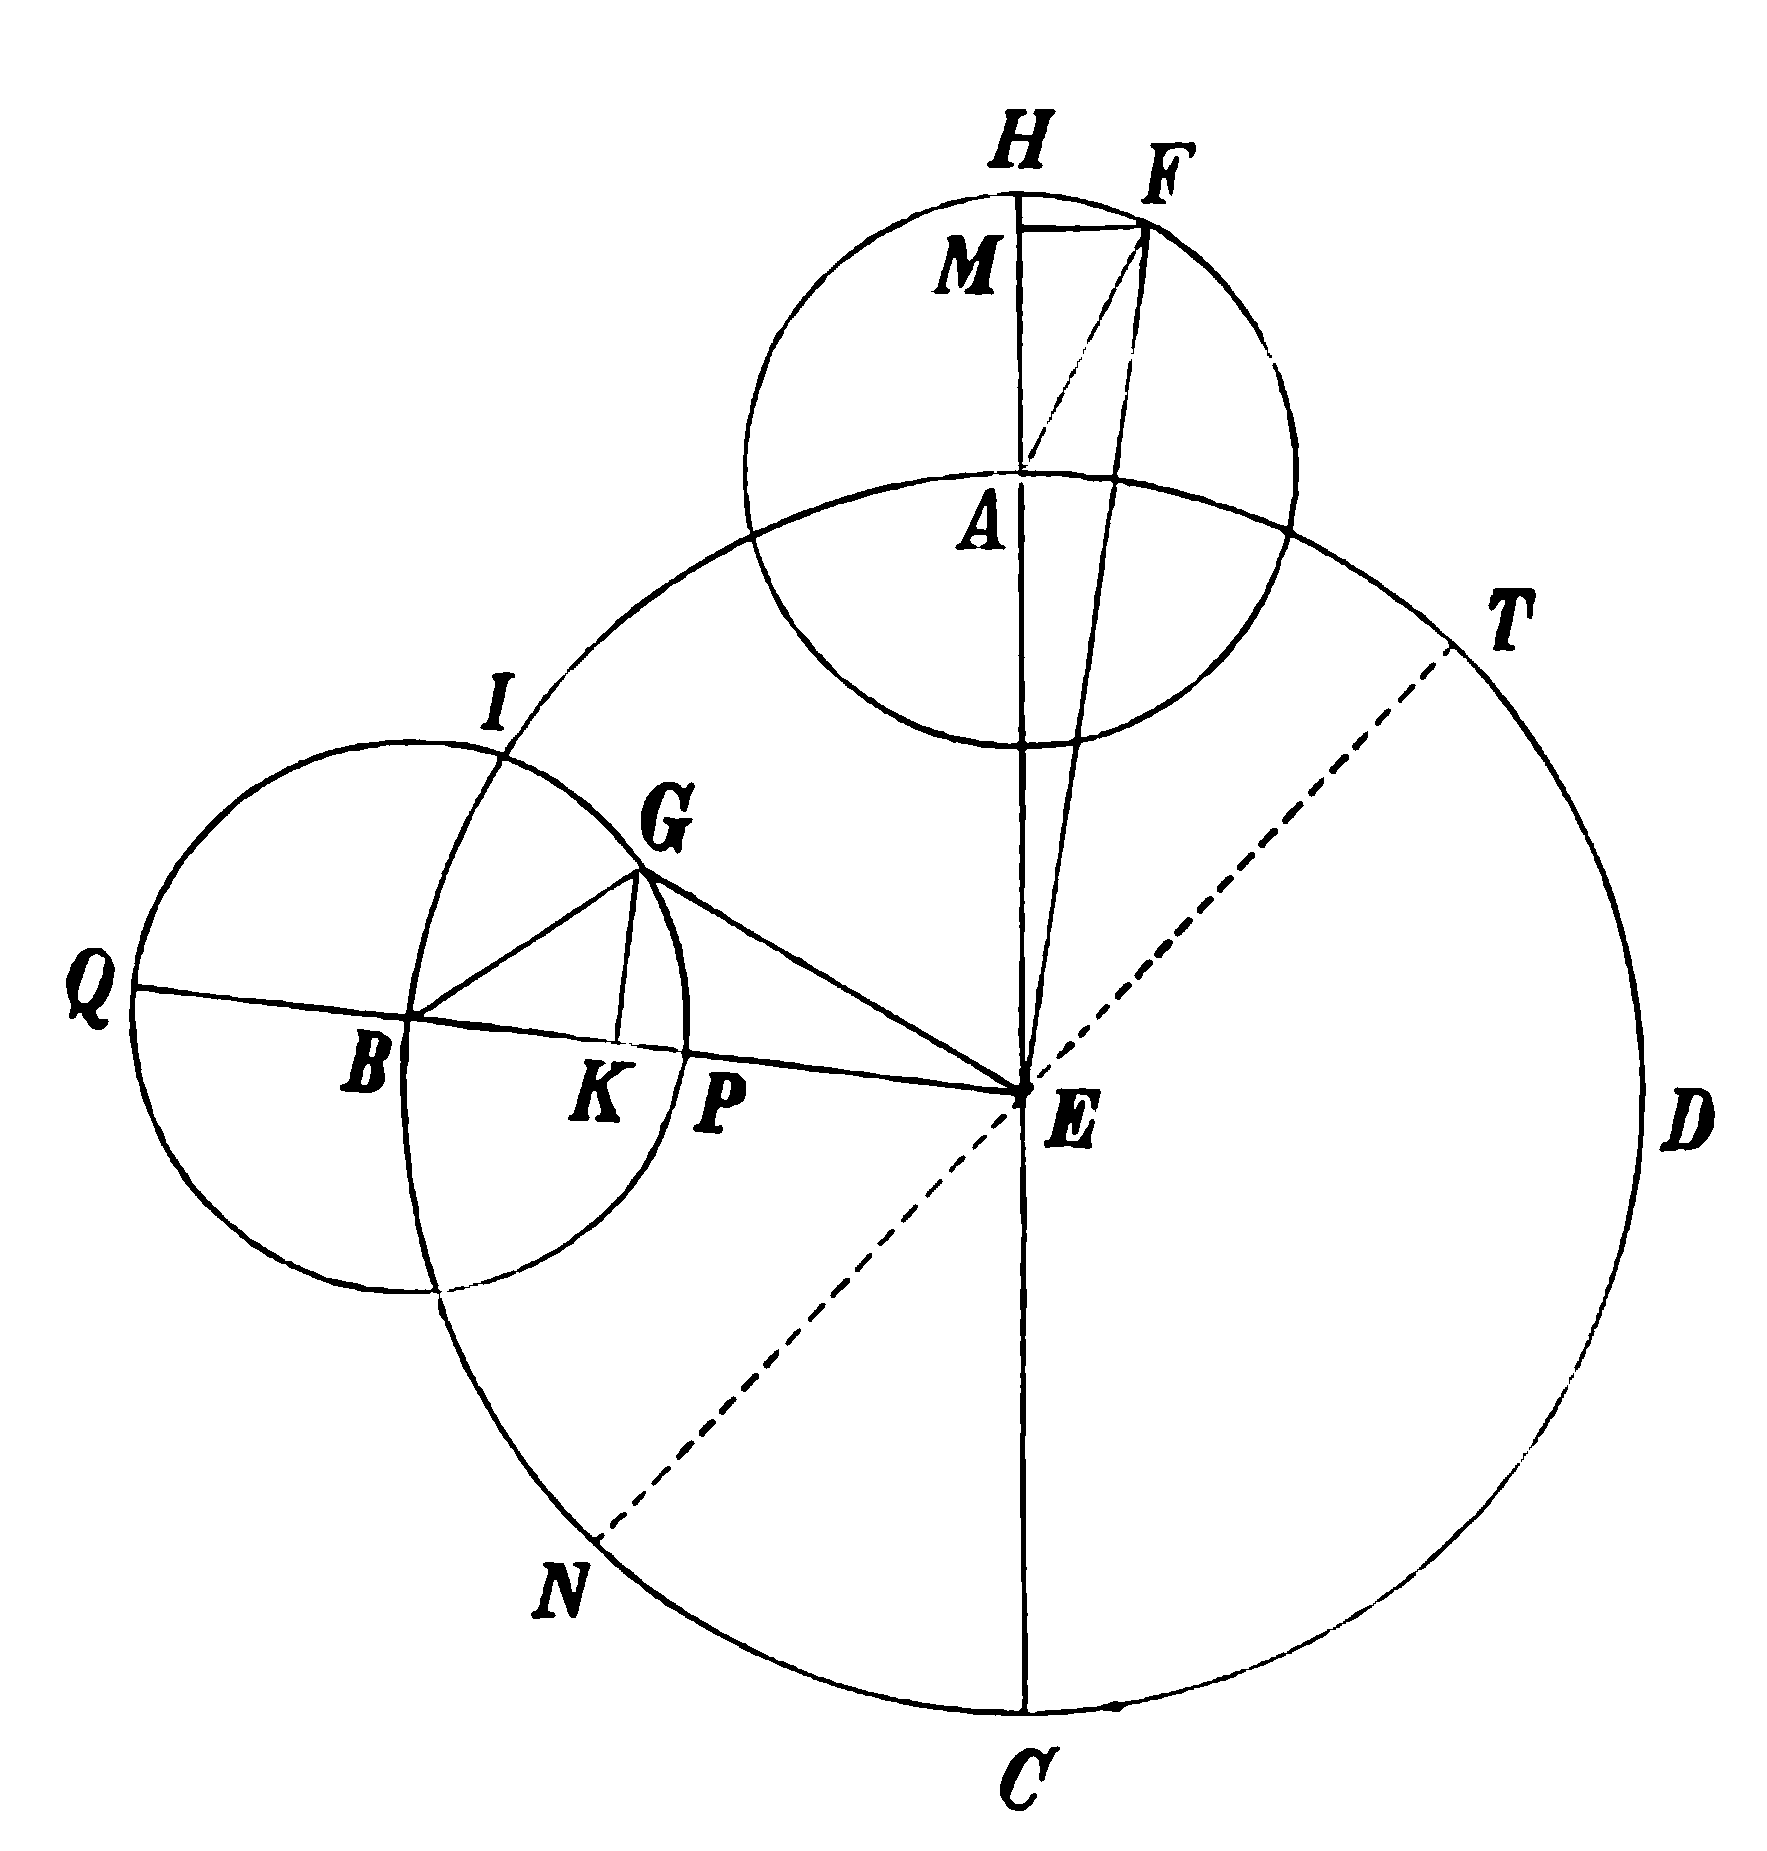
\includegraphics[width=\linewidth]{AB01-PDF0135-F01.png}\end{minipage}\hfill\begin{minipage}[t]{0.465\FullSourceWidth}\vspace{0pt}\setlength{\GutterOffset}{0.5349999999999999\FullSourceWidth}
\DLine{AB01-PDF0135-body-L018}{}{}{cognoscuntur] (9). Cum arcus GP, ut posui-}
\DLine{AB01-PDF0135-body-L019}{}{}{mus, $30^\circ$ contineat, eius sinus quoque $30^p$}
\DLine{AB01-PDF0135-body-L020}{20}{}{erit; arcus autem complementaris, qui su-}
\DLine{AB01-PDF0135-body-L021}{}{}{per KB est, sinum habebit $51^p57'41''$ (10).}
\DLine{AB01-PDF0135-body-L022}{}{}{--- At ex partibus quarum linea BG $2^p4'\,\qfrac{3}{4}$}
\DLine{AB01-PDF0135-body-L023}{}{}{habet, perpendicularis KG $1^p2'22''\,\qfrac{1}{2}$ (11)}
\DLine{AB01-PDF0135-body-L024}{}{}{continebit; remanet linea KB $1^p48'2''$, qua}
\DLine{AB01-PDF0135-body-L025}{25}{}{re EK fere $58^p11'58''$, et EG fere $58^p12'$}
\DLine{AB01-PDF0135-body-L026}{}{}{$34''$ (12) continebit ({\itshape e}). Sed ex partibus qua-}
\DLine{AB01-PDF0135-body-L027}{}{}{rum EG 60 habet, cathetus KG $1^p4'17''$ (13)}
\DLine{AB01-PDF0135-body-L028}{}{}{complectetur, et arcus super eam positus}
\DLine{AB01-PDF0135-body-L029}{}{}{$1^\circ1'24''$ (14), iuxta rationem qua circulus}
\DLine{AB01-PDF0135-body-L030}{30}{}{triangulum rectangulum BKG circumdans}
\DLine{AB01-PDF0135-body-L031}{}{}{in $360^\circ$ dividitur. Et hic est arcus anoma-}
\DLine{AB01-PDF0135-body-L032}{}{}{liae, scilicet arcus PG. Qua re arcus NB (15)}
\DLine{AB01-PDF0135-body-L033}{}{}{eclipticae, quem cognoscere volebamus, $31^\circ$}\end{minipage}\par
\DLine{AB01-PDF0135-body-L034}{}{}{$1'24''$ (16) complectetur.}
\par\vspace{6pt}\hrule height.25pt\vspace{5pt}
\noindent\begin{minipage}[t]{.48\textwidth}\vspace{0pt}\fontsize{9}{11.5}\selectfont\setlength{\GutterOffset}{0pt}
\hypertarget{AB01-PDF0135-N01}{}
\DLine{AB01-PDF0135-notes_left-L001}{}{}{\Indent (1) Cod.: « quod est quod angulo FAH et arcui}
\DLine{AB01-PDF0135-notes_left-L002}{}{}{« FH deest ad quadrantem perficiendum ».}
\hypertarget{AB01-PDF0135-N02}{}
\DLine{AB01-PDF0135-notes_left-L003}{}{}{\Indent (2) Pro $22''$ Plato habet $55''$. Persaepe in Pla-}
\DLine{AB01-PDF0135-notes_left-L004}{}{}{tonis editione pro 2 legitur 5, qui error codicibus}
\DLine{AB01-PDF0135-notes_left-L005}{}{}{Latinis vel editoris incuriae tribuendus est.}
\hypertarget{AB01-PDF0135-N03}{}
\DLine{AB01-PDF0135-notes_left-L006}{}{}{\Indent (3) Codex EF.}
\hypertarget{AB01-PDF0135-N04}{}
\DLine{AB01-PDF0135-notes_left-L007}{}{}{\Indent (4) Plato verba seqq. omittit et pro $2''$ habet $35''$.}
\hypertarget{AB01-PDF0135-N05}{}
\DLine{AB01-PDF0135-notes_left-L008}{}{}{\Indent (5) Plato $1^\circ33'$.}
\hypertarget{AB01-PDF0135-N06}{}
\DLine{AB01-PDF0135-notes_left-L009}{}{}{\Indent (6) Cod. QM.}
\hypertarget{AB01-PDF0135-N07}{}
\DLine{AB01-PDF0135-notes_left-L010}{}{}{\Indent (7) Male Plato 120.}
\hypertarget{AB01-PDF0135-N08}{}
\DLine{AB01-PDF0135-notes_left-L011}{}{}{\Indent (8) Cod.: eclipticae.}
\hypertarget{AB01-PDF0135-N09}{}
\DLine{AB01-PDF0135-notes_left-L012}{}{}{\Indent (9) Addidi, Platonem sequens; sed additio non}
\DLine{AB01-PDF0135-notes_left-L013}{}{}{est necessaria.}
\end{minipage}
\hfill\begin{minipage}[t]{.48\textwidth}\vspace{0pt}\fontsize{9}{11.5}\selectfont\setlength{\GutterOffset}{0pt}
\hypertarget{AB01-PDF0135-N10}{}
\DLine{AB01-PDF0135-notes_right-L001}{}{}{\Indent (10) Partes apud Plat. $59^p$.}
\hypertarget{AB01-PDF0135-N11}{}
\DLine{AB01-PDF0135-notes_right-L002}{}{}{\Indent (11) Deest $\qfrac{1}{2}$ in cod.; Plato pro $22''$ habet $55''$}
\DLine{AB01-PDF0135-notes_right-L003}{}{}{(cfr. adnot. 2).}
\hypertarget{AB01-PDF0135-N12}{}
\DLine{AB01-PDF0135-notes_right-L004}{}{}{\Indent (12) Plato $58^p7'34''$.}
\hypertarget{AB01-PDF0135-N13}{}
\DLine{AB01-PDF0135-notes_right-L005}{}{}{\Indent (13) Secundae apud Platonem $13''$.}
\hypertarget{AB01-PDF0135-N14}{}
\DLine{AB01-PDF0135-notes_right-L006}{}{}{\Indent (14) Plato $1^p4'54''$.}
\hypertarget{AB01-PDF0135-N15}{}
\DLine{AB01-PDF0135-notes_right-L007}{}{}{\Indent (15) Cod. IB (\textarabic{ى} I pro \textarabic{ن} N); Plato GB. In figura}
\DLine{AB01-PDF0135-notes_right-L008}{}{}{codicis et Platonis punctum N lineaque NT desunt;}
\DLine{AB01-PDF0135-notes_right-L009}{}{}{punctum T vero, ut supra notavi, perperam prope}
\DLine{AB01-PDF0135-notes_right-L010}{}{}{locum intersectionis epicycli HF et eclipticae collo-}
\DLine{AB01-PDF0135-notes_right-L011}{}{}{catum.}
\hypertarget{AB01-PDF0135-N16}{}
\DLine{AB01-PDF0135-notes_right-L012}{}{}{\Indent (16) Minuta in cod. $4'$; Plat. $1^\circ4'54''$.}
\end{minipage}

\DSource{0136}{47}
\hypertarget{AB01-PDF0136-P01}{}
\DLine{AB01-PDF0136-body-L001}{}{}{\Indent Dicit [auctor]: Nunc aliter haec explicabimus. Circa centrum E et diametrum AC, sit}
\DLine{AB01-PDF0136-body-L002}{}{}{circulus eclipticae ABC; circa centrum H, excentricus FMG; et diametrus AC per ambo}
\DLine{AB01-PDF0136-body-L003}{}{p. 71.}{centra transeat. Erit F punctum apogei in circulo parecliptico, G perigei. Initio locum Solis}
\DLine{AB01-PDF0136-body-L004}{}{}{in excentrico in M esse ponamus, et arcum FM excentrici, quem Sol iam percurrit, $30^\circ$ com-}
\DLine{AB01-PDF0136-body-L005}{5}{}{plecti; angulus FHM erit quoque $30^\circ$. Lineam EH, ambo centra coniungentem, iam vidimus}
\DLine{AB01-PDF0136-body-L006}{}{}{$2^p4'\,\qfrac{3}{4}$ esse. Semidiametrum HM excentrici et lineam EM ducamus, HM usque ad punctum}
\DLine{AB01-PDF0136-body-L007}{}{}{L quo cum perpendiculari LE convenit protrahentes. Triangulum HLE rectangulum est; eius}
\DLine{AB01-PDF0136-body-L008}{}{}{angulus LHE aequat angulum datum FHM; arcus super EL, ex circulo triangulum HLE}
\DLine{AB01-PDF0136-body-L009}{}{}{circumdanti, si circumferentia $360^\circ$ continet, $30^\circ$ complectetur, eiusque sinus $30^p$ quoque ex}
\DLine{AB01-PDF0136-body-L010}{10}{}{partibus quarum linea HE inter ambo centra 60 habet. Remanebit linea LH, quadrantem per-}
\DLine{AB01-PDF0136-body-L011}{}{}{ficiens, $51^p57'41''$, nam arcus complementaris LH $60^\circ$ continet. Sed ea ratione qua linea HE}
\DLine{AB01-PDF0136-body-L012}{}{}{inter ambo centra $2^p4'\,\qfrac{3}{4}$ complectitur, linea EL $1^p2'22''\,\qfrac{1}{2}$ (1) erit, et linea LH, quadran-}
\DLine{AB01-PDF0136-body-L013}{}{}{tem perficiens, $1^p48'2''$; itaque linea tota LM $61^p48'2''$. Triangulum MLE rectangulum est;}
\DLine{AB01-PDF0136-body-L014}{}{}{eius hypotenusam EM $61^p48'35''$ esse vidimus. Sed ratione qua lineae EM $60^p$ tribuuntur,}
\DLine{AB01-PDF0136-body-L015}{15}{}{EL est $1^p33'$ (2), et arcus super eam $0^\circ57'49''$, cum circulus triangulum HLE circumdans}
\DLine{AB01-PDF0136-body-L016}{}{}{$360^\circ$ sit. Arcus igitur AB eclipticae $29^\circ2'11''$ fere remanebit.}
\hypertarget{AB01-PDF0136-P02}{}
\DLine{AB01-PDF0136-body-L017}{}{}{\Indent Item Solem in puncto D excentrici esse ponamus, arcumque FD (3) $150^\circ$ complecti; reli-}
\DLine{AB01-PDF0136-body-L018}{}{}{quus arcus DG, inter locum Solis et perigeum, $30^\circ$ erit. Lineas EK et HD, quarum utraque}
\DLine{AB01-PDF0136-body-L019}{}{}{est sui circuli semidiametrus, ducamus; item perpendicularem ES. Triangulum HSE rectan-}
\DLine{AB01-PDF0136-body-L020}{20}{}{gulum est; latus EH, ambo centra coniungens, latus ES, angulus DHG (4) nota sunt; erunt}
\DLine{AB01-PDF0136-body-L021}{}{}{ergo nota latus HS et angulus HES (5). Cognoscuntur igitur quoque linea DG et hypotenusa}
\DLine{AB01-PDF0136-body-L022}{}{}{ED trianguli rectanguli ESD. Cum vero datus arcus DG et datus angulus GHD $30^\circ$ sint ut}
\DLine{AB01-PDF0136-body-L023}{}{}{diximus, eorumque sinus $30^p$ pariter, arcus quoque ES circuli triangulum rectangulum ESH}
\DLine{AB01-PDF0136-body-L024}{}{}{circumdantis complectetur $30^\circ$ ex partibus quarum totus ille circulus $360^\circ$ habet, et eius sinus,}
\DLine{AB01-PDF0136-body-L025}{25}{p. 72.}{nempe cathetus ES, $30^p$ quoque e partibus quarum linea EH, semidiametrus huius circuli, $60^p$}
\DLine{AB01-PDF0136-body-L026}{}{}{complectitur. Sed ratione qua lineae EH $2^p4'\,\qfrac{3}{4}$ tribuuntur, cathetus ES erit $1^p2'22''\,\qfrac{1}{2}$ (6);}
\par\noindent\begin{minipage}[t]{0.54\FullSourceWidth}\vspace{0pt}\centering\hypertarget{AB01-PDF0136-F01}{}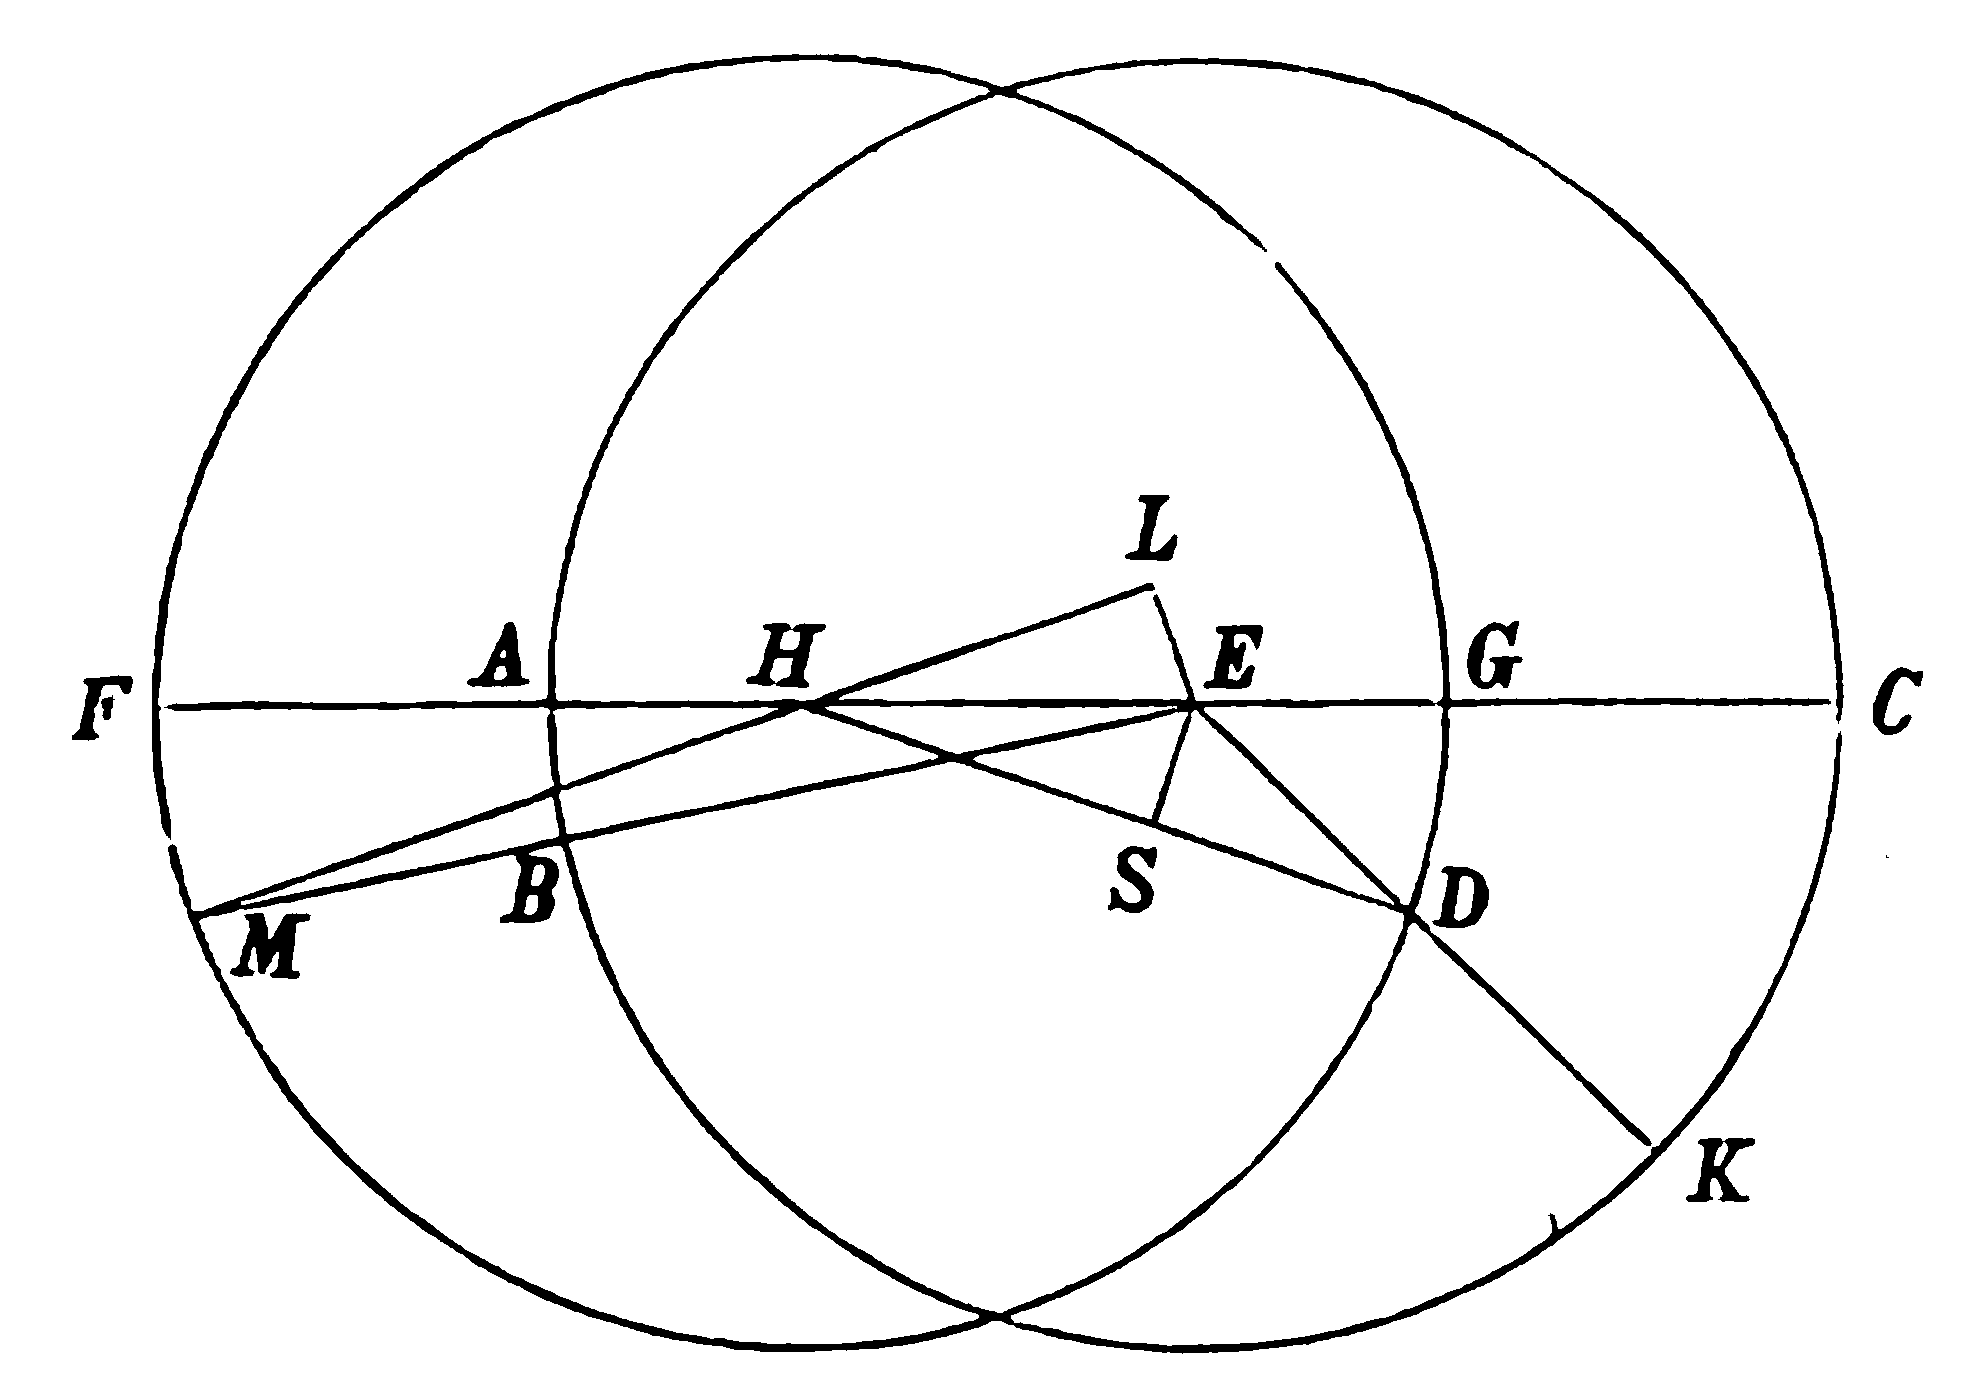
\includegraphics[width=\linewidth]{AB01-PDF0136-F01.png}\end{minipage}\hfill\begin{minipage}[t]{0.43\FullSourceWidth}\vspace{0pt}\setlength{\GutterOffset}{0.5700000000000001\FullSourceWidth}
\DLine{AB01-PDF0136-body-L027}{}{}{qua re latus SH $1^p48'2''$ remanebit.}
\DLine{AB01-PDF0136-body-L028}{}{}{Semidiametrus HD excentrici $60^p$ conti-}
\DLine{AB01-PDF0136-body-L029}{}{}{net, de quibus si SH dematur, remanent}
\DLine{AB01-PDF0136-body-L030}{30}{}{lineae SD $58^p11'58''$; igitur hypote-}
\DLine{AB01-PDF0136-body-L031}{}{}{nusa ED trianguli rectanguli ESD erit}
\DLine{AB01-PDF0136-body-L032}{}{}{circiter $58^p12'32''$ (7). Sed ex partibus}
\DLine{AB01-PDF0136-body-L033}{}{}{quarum linea ED 60 habet, cathetus ES}
\DLine{AB01-PDF0136-body-L034}{}{}{$1^p4'17''$ complectetur, et arcus super}
\DLine{AB01-PDF0136-body-L035}{35}{}{eam, qui est quantitas anomaliae, $1^\circ1'$}
\DLine{AB01-PDF0136-body-L036}{}{}{$24''$ (8): arcus igitur KC eclipticae, $31^\circ$}
\DLine{AB01-PDF0136-body-L037}{}{}{$1'24''$ (9) circiter erit. Haec de anomalia}
\DLine{AB01-PDF0136-body-L038}{}{}{sufficiunt, quam explicare volebamus.}
\hypertarget{AB01-PDF0136-P03}{}
\DLine{AB01-PDF0136-body-L039}{}{}{\Indent Dicit [auctor]: Hunc motum ita ad}\end{minipage}\par
\DLine{AB01-PDF0136-body-L040}{40}{}{singulos gradus in tabulis a puncto apogei posuimus; similiter reperiuntur aequatio simplex}
\par\vspace{6pt}\hrule height.25pt\vspace{5pt}
\noindent\begin{minipage}[t]{.48\textwidth}\vspace{0pt}\fontsize{9}{11.5}\selectfont\setlength{\GutterOffset}{0pt}
\hypertarget{AB01-PDF0136-N01}{}
\DLine{AB01-PDF0136-notes_left-L001}{}{}{\Indent (1) Secundae apud Platonem $55''$.}
\hypertarget{AB01-PDF0136-N02}{}
\DLine{AB01-PDF0136-notes_left-L002}{}{}{\Indent (2) Cod. « unius partis et trium ac triginta se-}
\DLine{AB01-PDF0136-notes_left-L003}{}{}{« cundarum ».}
\hypertarget{AB01-PDF0136-N03}{}
\DLine{AB01-PDF0136-notes_left-L004}{}{}{\Indent (3) Cod. AD. Postea Plato 120.}
\hypertarget{AB01-PDF0136-N04}{}
\DLine{AB01-PDF0136-notes_left-L005}{}{}{\Indent (4) Cod. HDG.}
\end{minipage}
\hfill\begin{minipage}[t]{.48\textwidth}\vspace{0pt}\fontsize{9}{11.5}\selectfont\setlength{\GutterOffset}{0pt}
\hypertarget{AB01-PDF0136-N05}{}
\DLine{AB01-PDF0136-notes_right-L001}{}{}{\Indent (5) Cod. HS.}
\hypertarget{AB01-PDF0136-N06}{}
\DLine{AB01-PDF0136-notes_right-L002}{}{}{\Indent (6) Secundae apud Platonem $55''$.}
\hypertarget{AB01-PDF0136-N07}{}
\DLine{AB01-PDF0136-notes_right-L003}{}{}{\Indent (7) Plato $58^p15'34''$. Cfr. adnot. {\itshape e} huius capitis.}
\hypertarget{AB01-PDF0136-N08}{}
\DLine{AB01-PDF0136-notes_right-L004}{}{}{\Indent (8) Cod. $1^\circ4'24''$; Plato $1^\circ4'54''$.}
\hypertarget{AB01-PDF0136-N09}{}
\DLine{AB01-PDF0136-notes_right-L005}{}{}{\Indent (9) Cod. $1^\circ1'24''$; Plato $31^\circ4'54''$.}
\end{minipage}

\DSource{0137}{48}
\hypertarget{AB01-PDF0137-P01}{}
\DLine{AB01-PDF0137-body-L001}{}{}{Lunae et aequatio media quinque planetarum, quae est semidiametrus eorum epicycli, cum}
\DLine{AB01-PDF0137-body-L002}{}{}{eius sinus sumatur et eo modo dividatur.}
\hypertarget{AB01-PDF0137-P02}{}
\DLine{AB01-PDF0137-body-L003}{}{}{\Indent Si id calculo reperire vis, gradus epicycli quos ab apogeo Sol, vel Luna, vel planeta}
\DLine{AB01-PDF0137-body-L004}{}{}{percurrerit, scilicet anomaliam, observa; si gradus minus quam $180^\circ$ sunt, iis utere, sed si}
\DLine{AB01-PDF0137-body-L005}{}{}{$180^\circ$ superant, eos de $360^\circ$ deme et residuum adhibe. Graduum alterutra via repertorum, si}
\DLine{AB01-PDF0137-body-L006}{5}{}{minus quam $90^\circ$ sunt, sinum atque cosinum multiplica in semidiametrum epicycli sideris qui}
\DLine{AB01-PDF0137-body-L007}{}{}{est totius aequationis sinus; ambo producta per semidiametrum divide, et quod ex divisione}
\DLine{AB01-PDF0137-body-L008}{}{p. 73.}{cosinus provenerit adde $60^p$ scilicet semidiametro. Quadratum huius summae adde quadrato}
\DLine{AB01-PDF0137-body-L009}{}{}{eius quod e divisione sinus exierit; huius summae radicem inveni. Deinde quod e divisione}
\DLine{AB01-PDF0137-body-L010}{}{}{sinus provenerat, in semidiametrum multiplica, et productum per inventam radicem divide. ---}
\DLine{AB01-PDF0137-body-L011}{10}{}{Si contra gradus adhibendi superant $90^\circ$, de iis $90^\circ$ deme; sinum et cosinum residui in semi-}
\DLine{AB01-PDF0137-body-L012}{}{}{diametrum epicycli multiplica et per semidiametrum divide; quod e sinu provenerit de $60^p$}
\DLine{AB01-PDF0137-body-L013}{}{}{deme; quadratum residui adde quadrato eius quod e cosinu exierit, et huius summae radi-}
\DLine{AB01-PDF0137-body-L014}{}{}{cem inveni. Postea quod e divisione cosinus provenerat in semidiametrum multiplica, et pro-}
\DLine{AB01-PDF0137-body-L015}{}{}{ductum per radicem inventam divide. --- Quod ex alterutra operatione tibi provenerit, in}
\DLine{AB01-PDF0137-body-L016}{15}{}{arcum converte; arcus erit portio graduum ad anomaliam qua usus es pertinens, scilicet ae-}
\DLine{AB01-PDF0137-body-L017}{}{}{quatio stellae ({\itshape f}).}
\hypertarget{AB01-PDF0137-P03}{}
\DLine{AB01-PDF0137-body-L018}{}{}{\Indent Semidiametrus epicycli Solis est $2^p4'45''$ (1); semidiametrus epicycli Lunae $5^p15'$ (2);}
\DLine{AB01-PDF0137-body-L019}{}{}{Saturni $6^p29'50''$ (3); Iovis $11^p30'0''$ (4); Martis $39^p27'22''$ (5); Veneris $43^p9'0''$ (6); Mer-}
\DLine{AB01-PDF0137-body-L020}{}{}{curii $22^p30'30''$ (7). Hoc ex observationibus patuit et cum calculis congruit; idque, volente}
\DLine{AB01-PDF0137-body-L021}{20}{}{Deo, est sinus aequationis mediae ({\itshape g}).}
\vspace{27.6pt}
\hypertarget{AB01-PDF0137-H01}{}
\DLine{AB01-PDF0137-body-L022}{}{}{\CenterLine{CAPUT XXIX.}}
\vspace{13.8pt}
\DLine{AB01-PDF0137-body-L023}{25}{}{\CenterLine{De inaequalitate nychthemerōn et de aliorum in alia conversione.}}
\vspace{13.8pt}
\hypertarget{AB01-PDF0137-P04}{}
\DLine{AB01-PDF0137-body-L024}{}{}{\Indent Dicit [auctor]: Plurimi homines et vulgus nychthemera existimant aequalia esse, et eo-}
\DLine{AB01-PDF0137-body-L025}{}{}{rum quodque 24 horas amplecti; sed hoc haud verum est, nam nychthemerum medium est}
\DLine{AB01-PDF0137-body-L026}{}{p. 74.}{ortus omnium 360 temporum aequatoris ab horizonte vel a circulo meridiano, eo addito quod}
\DLine{AB01-PDF0137-body-L027}{30}{}{ex aequatoris temporibus ascendit cum 59 minutis quae Sol, motu suo medio, in nychthemero}
\DLine{AB01-PDF0137-body-L028}{}{}{percurrit. Nychthemerum autem inaequale est ortus 360 temporum aequatoris, addito motu}
\DLine{AB01-PDF0137-body-L029}{}{}{inaequali Solis in nychthemero, qui necessarie minor aut maior est quam $59'$.}
\hypertarget{AB01-PDF0137-P05}{}
\DLine{AB01-PDF0137-body-L030}{}{}{\Indent Quoniam omni loco initium a circulo horizontis variat prout in illo variant ascensiones}
\DLine{AB01-PDF0137-body-L031}{}{}{signorum, initium autem ab hora meridiana immobile est neque mutatur, ob aequalitatem}
\DLine{AB01-PDF0137-body-L032}{35}{}{ascensionum signorum in circulo meridiano quolibet loco, in calculo stellarum earumque lo-}
\DLine{AB01-PDF0137-body-L033}{}{}{corum initium diei non ponitur ab ortu vel occasu Solis, sed a tempore meridiei aut mediae}
\DLine{AB01-PDF0137-body-L034}{}{}{noctis (8) ({\itshape a}).}
\hypertarget{AB01-PDF0137-P06}{}
\DLine{AB01-PDF0137-body-L035}{}{}{\Indent Item quoniam omnes motus stellarum in tabulis nonnisi ad aequales dies supputantur,}
\DLine{AB01-PDF0137-body-L036}{}{}{differentia inter nychthemera inaequalia et nychthemera media negligitur. In motu Solis et}
\DLine{AB01-PDF0137-body-L037}{40}{}{reliquarum stellarum differentia tanta non est ut errorem sensibilem gignat; sed error mani-}
\par\vspace{6pt}\hrule height.25pt\vspace{5pt}
\noindent\begin{minipage}[t]{.48\textwidth}\vspace{0pt}\fontsize{9}{11.5}\selectfont\setlength{\GutterOffset}{0pt}
\hypertarget{AB01-PDF0137-N01}{}
\DLine{AB01-PDF0137-notes_left-L001}{}{}{\Indent (1) Cod. $5'$ pro $4'$.}
\hypertarget{AB01-PDF0137-N02}{}
\DLine{AB01-PDF0137-notes_left-L002}{}{}{\Indent (2) Gradus in cod. $6^\circ$.}
\hypertarget{AB01-PDF0137-N03}{}
\DLine{AB01-PDF0137-notes_left-L003}{}{}{\Indent (3) Secundae apud Plat. $7''$.}
\hypertarget{AB01-PDF0137-N04}{}
\DLine{AB01-PDF0137-notes_left-L004}{}{}{\Indent (4) Secundae apud Plat. $5''$.}
\end{minipage}
\hfill\begin{minipage}[t]{.48\textwidth}\vspace{0pt}\fontsize{9}{11.5}\selectfont\setlength{\GutterOffset}{0pt}
\hypertarget{AB01-PDF0137-N05}{}
\DLine{AB01-PDF0137-notes_right-L001}{}{}{\Indent (5) Cod. $19^\circ25'22''$; minuta apud Plat. $55'$.}
\hypertarget{AB01-PDF0137-N06}{}
\DLine{AB01-PDF0137-notes_right-L002}{}{}{\Indent (6) Plat. $44^\circ9'5''$.}
\hypertarget{AB01-PDF0137-N07}{}
\DLine{AB01-PDF0137-notes_right-L003}{}{}{\Indent (7) Gradus in cod. $29^\circ$.}
\hypertarget{AB01-PDF0137-N08}{}
\DLine{AB01-PDF0137-notes_right-L004}{}{}{\Indent (8) {\itshape Almag.} III, 8 (ed. Halma, t. I, p. 208).}
\end{minipage}
\end{document}
